

\section{Reconstruction code}


The energy deposited by the particles in the towers produces scintillating light that is propagated with optic fibers through the different layers to APD placed at the base of the cells. The APDs amplify the signal and generate an electronic pulse shape that is stored in the raw data format. From this pulse shape, we extract the signal amplitude and the arrival time. The pulse shape is fitted during the reconstruction via a parametrized function and TMinuit, and those 2 values are extracted.

A particle produces signals in different towers (electromagnetic shower expands more than its Moli\`ere radius which is a cell size). The next step is the formation of clusters of cells that belong to the same particle, although depending on the energy, granularity, clusterization algorithm or event type, those clusters might have contributions from different particles. The default algorithm in pp collisions is a simple aggregation of neighboring cells until there is no more cells above a certain energy threshold (named {\it clusterizer V1}). In case of Pb-Pb collisions environment, where particle showers merge quite often, we apply another algorithm that aggregates cells to the clusters until reaching a cell with more energy than the precedent (named {\it clusterizer V2}). Depending on the analysis type, one might want to use one or the other clusterization type. For this reason, a re-clusterization is also possible at the analysis level. A last clusterizer is implemented, which makes 3x3 clusters. It has been used in jet analysis for instance in order to avoid biasing jet reconstruction where one is interested in the energy flow over a large area without explicit reconstruction of photon showers and where the driving consideration is that the wide clusterizer does not interfere with the jet finder. For $\pi^{0}$, $\eta$, and direct $\gamma$ analyses, {\it V2} is most likely preferable).

Once the cluster is defined, we calculate cluster parameters, shower shape parameters, that will help at the analysis level to identify each cluster as one particle type. Also, we compare the cluster position information with the propagation of tracks measured in the central barrel to the EMCAL surface, to identify the clusters generated by charged particles.

The final analysis objects, ESDs and AODs, contain all the cluster and cell basic informations allowing to redo the clusterization if needed at the analysis level.

%The class AliReconstruction manages this part. This step can
%begin either from the Digits or from the Raw data. We can distinguish
%different steps described in the following sections. 


\subsection{Offline data base access}

How to create explained OCDB/OADB section.

\subsubsection{Energy calibration}

\subsubsection{Bad channels - Marie, Alexis}

\subsubsection{Alignment - Marco}

\subsection{Raw data fitting: from ADC sample to digits - David}

As also discussed in Sec.~\ref{sec:simu_raw}, the recorded Raw data consists
of instead a series of so-called time samples with 10-bit ADC counts per channel. 
Each time bin is 100 ns wide, corresponding to a 10 MHz readout.
The expected signal (Gamma-2) shape is described e.g. in the AliEMCALRawResponse class,
in the RawResponseFunction method.
The reconstruction from Raw data to Digits is done in the AliEMCALRawUtils class,
Raw2Digits method.
The Raw ADC time samples data is kept in AliCaloBunchInfo objects, which are given
as input to an AliCaloRawAnalyzer object, which returns the signal amplitude and time
information (in the form of an AliCaloFitResults object).
There are several different AloCaloRawAnalyzer versions, which can be selected via
AliEMCALRawUtils::SetFittingAlgorithm(). They are:

\begin{itemize}
 \item kStandard:
   AliCaloRawAnalyzerKStandard, which is a (slower but simple) Gamma-2 fit implementation.
 \item  kFastFit: 
   AliCaloRawAnalyzerFastFit, which is a faster Gamma-2 fit implementation from Aleksei Pavlinov.
 \item kNeuralNet:
   AliCaloRawAnalyzerNN, which is a neural network implementation from Paola La Rocca and Franco Riggi.
 \item kPeakFinder:
   AliCaloRawAnalyzerPeakFinder, which is a fast (parameterized vector operations) implementation from Per Thomas Hille. 
 \item kCrude:
   AliCaloRawAnalyzerCrude, which is the simplest possible algorithm: just take the maximum ADC value as the signal amplitude.
 \item kFakeAltro:
   AliCaloRawAnalyzerFakeALTRO, which is an algorithm intended for the Trigger/TRU raw data analysis, i.e. not for the regular FEE or cell/tower data.
\end{itemize}



\subsection{Clusterization: From digits to clusters - Adam}


%\subsection{Clusterization: From digits to clusters -  Adam}
%classes:
%AliEMCALClusterizer.cxx
%AliEMCALClusterizerv1.cxx
%AliEMCALClusterizerNxN.cxx
%AliEMCALClusterizerv2.cxx
%AliEMCALClusterizerFixedWindow.cxx  
%unfolding
The set of information related to one cell - (between each other) the position of cell and the energy deposited in it is called a digit. The digit is represented by the \texttt{AliEMCALDigit} class. A group of digits which are related somehow between each other is called a cluster. The cluster is represented by the \texttt{AliEMCALRecPoint} class.

Transformation from digits to clusters is done during clusterization phase. There are many ideas how to form cluster. Each applied idea is called clusterizer. Currently, there are four types of clusterizers in the EMCal:

%\parskip

\begin{itemize}
%\parskip
\item Clusterizer V1,
\item Clusterizer V2.
\item Clusterizer V1 with unfolding,
\item Clusterizer NxN,

\end{itemize}


Technically it is organized in the following way. \texttt{AliEMCALClusterizer} is a base clusterizer class. The V1 and NxN clusterizer classes (\texttt{AliEMCALClusterizerv1} and \texttt{AliEMCALClusterizerNxN}, respectively) inherit from the base class. The clusterizer class V2 (\texttt{AliEMCALClusterizerv2}) inherits from \texttt{AliEMCALClusterizerv1}. The third case of clusterization (clusterizer V1 with unfolding) is realized via settable option in the \texttt{AliEMCALClusterizerv1} class. The dedicated class \texttt{AliEMCALUnfolding} was written for the purpose of unfolding. The description of each clusterizer type separately and common clusterization structure together with a description of the cluster is explained below.
\subsubsection{Clusterization in the EMCal}
A clusterizer is called in the \texttt{AliEMCALReconstructor} class. The set of clusterizer parameters is initialised. Usually parameters are taken from the OCDB. The full set of parameters which are used during clusterization is given in Tab.~\ref{tab:clusterizationparams}. The other fields of the \texttt{AliEMCALClusterizer} class are given in Tab.~\ref{tab:clusterizationfields}.
%
\begin{table}[!h]
\begin{center}
  \begin{tabular}{| c | c | l |}
  \hline
  Name & Type & Explanation \\ 
  \hline
   fTimeMin                & \texttt{Float\_t } & minimum time of physical signal in a cell/digit\\
   fTimeMax                & \texttt{Float\_t } & maximum time of physical signal in a cell/digit\\
   fTimeCut                & \texttt{Float\_t } & maximum time difference between the digits inside EMC cluster\\
   fToUnfold               & \texttt{Bool\_t  } & says if unfolding should be performed \\
   fECAClusteringThreshold & \texttt{Float\_t } & minimum energy to seed a EC digit in a cluster\\
   fECALocMaxCut           & \texttt{Float\_t } & minimum energy difference to distinguish local maxima in a cluster\\
   fECAW0                  & \texttt{Float\_t } & logarithmic weight for the cluster center of gravity calculation\\
   fMinECut                & \texttt{Float\_t } & minimum energy for a digit to be a member of a cluster\\
   fSSPars[8]              & \texttt{Double\_t} & shower shape parameters \\
   fPar5[3]                & \texttt{Double\_t} & shower shape parameter 5\\
   fPar6[3]                & \texttt{Double\_t} & shower shape parameter 6\\
  \hline
  \end{tabular}
\end{center}
\caption{Parameter name, type and explanation.}
\label{tab:clusterizationparams}
\end{table}
%
\begin{table}[!h]
\begin{center}
  \begin{tabular}{| c | c | l |}
  \hline
  Name & Type & Explanation \\ 
  \hline
    fADCchannelECA     &  \texttt{Float\_t}         &  width of one ADC channel for EC section (GeV)\\
    fADCpedestalECA    &  \texttt{Float\_t}         &  pedestal of ADC for EC section (GeV)\\
    fTimeECA           &  \texttt{Float\_t}         &  calibration parameter for channels time\\
    fIsInputCalibrated &  \texttt{Bool\_t}          &  to enable reclusterization from ESD cells\\
    fJustClusters      &  \texttt{Bool\_t}          &  false for standard reco                  \\
    fDigitsArr    & \texttt{TClonesArray*}          &  pointer to array with EMCAL digits       \\
    fTreeR        & \texttt{TTree*}                 &  pointer to tree with output clusters                                         \\
    fRecPoints    & \texttt{TObjArray*}             &  pointer to array with EMCAL clusters                                         \\
    fGeom         & \texttt{AliEMCALGeometry*}      &  pointer to geometry for utilities                                            \\
    fCalibData    & \texttt{AliEMCALCalibData*}     &  pointer to calibration database if available                                  \\
    fCaloPed      & \texttt{AliCaloCalibPedestal*}  &  pointer to tower status map if available                                      \\
    fDefaultInit         & \texttt{Bool\_t}          &  says if the task was created by default ctor \\
    fNumberOfECAClusters & \texttt{Int\_t}           &  number of clusters found in EC section \\
    fClusterUnfolding & \texttt{AliEMCALUnfolding*} &  pointer to unfolding object \\
\hline
  \end{tabular}
\end{center}
\caption{Other fields in the \texttt{AliEMCALClusterizer} class.}
\label{tab:clusterizationfields}
\end{table}
%
Also input and output are connected. Finally, a clusterization phase is done in a \texttt{Digits2Clusters} method. Main steps run as follow:
\begin{enumerate}
\item Get calibration parameters (method \texttt{GetCalibrationParameters}),
\item Get pedestal parameters (method \texttt{GetCaloCalibPedestal}),
\item Make clusters (method \texttt{MakeClusters}),
\item Make unfolding or not (method \texttt{MakeUnfolding}),
\item Evaluate cluster properties (\texttt{AliEMCALRecPoint} class methods),
\item Store clusters.
\end{enumerate}
In the first two steps calibration (ADC counts to energy conversion) and pedestal parameters are read from a database. The third step, where clusters are formed, is different for each clusterizer. 
However, some beginning parts of this step are common for each algorithm. The input is the same. It is an array of fired digits with electronic signal registered in each of them. Also calibration and cleaning the array of digits, to work with reduced sample of digits, is the same for each algorithm. This common part is done in the common method \texttt{Calibrate} of the \texttt{AliEMCALClusterizer} class. Here, we require the proper timing (via selection of \texttt{fTimeMax} and \texttt{fTimeMin} of a given digit), status (check of dead channel map) and calibrate energy and time of each digit. If any digit fails to pass one of requirement it is rejected from a ``working array'' of digits (pool of digits). In make clusters step the \texttt{AreNeighbours} method is used. The method could differ for each clusterization algorithm. 
%Also the used method \texttt{AreNeighbours} differs for each clusterizer in this step. 
The explanation how clusters are formed is given in next four subsections for each clusterization algorithm, respectively. The next step (unfolding) is an option in each clusterizer, but currently is used only for the V1 clusterizer. The last two steps (evaluation of a cluster properties and its recording) are the same for each algorithm.

\subsubsection{Clusterizer V1}
%The input for each clusterizer is array of fired digits with electronic signal registered in each of them. The first step in each algorithm is to calibrate and clean array of digits to work with reduced sample of digits. It is done in common method \texttt{Calibrate} of \texttt{AliEMCALClusterizer} class. Here we require the proper timing (via selection of \texttt{fTimeMax} and \texttt{fTimeMin} of a given digit), status (check of dead channel map) and calibrate energy and time of each digit. If any digit fails to pass one of requirement it is rejected from a ``working array'' of digits. 
%Then, in the V1 algorithm, we reject digits with energy smaller than \texttt{fMinECut}, which is set to be by default 10~MeV in the database. 
Having obtained ``working array'' of digits in the V1 algorithm we additionally reject digits with energy smaller than \texttt{fMinECut}, which is set to be 10~MeV in the database by default.

After selecting digits we form clusters. We loop over all digits to find the first seed digit with energy grater than \texttt{fECAClusteringThreshold} (default value is 100~MeV). 
When the seed digit is found it is associated to a new cluster and removed from the ``working array'' of digits. We loop over all remaining digits to look for neighbours of the seed digit.
The neighbour digits are called digits which have at least common side (i.e.: row index difference or column index difference must be equal 1, but not both of them at the same time are equal 1, so one cell can have four neighbours at maximum).
The additional requirement on neighbour digits is applied. The absolute value of time difference for two digits must be less or equal \texttt{fTimeCut}.

The neighbour digits are associated to the cluster (also removed from the ``working array'' of digits) and we keep on looking for neighbours of each digit associated to the cluster. When a digit is associated to one cluster it cannot be associated to other one. When there are no more neighbours of digits in one cluster one can say that this cluster is formed. Once the cluster
is formed and there are still remaining digits in the ``working array'' the procedure starts to check seeds and all the story repeats until no seed digit is found. The consequence of such algorithm is that one cluster can contain all digits in the super-module. The other thing is that there can be digits which are not associated to any cluster. The special case when cluster is formed from digits in two super-modules at the same SM-$\phi$ angle is also supported.  



\subsubsection{Clusterizer V2}
%The first step in this algorithm is the same as in V1 clusterizer. It is calibration of digits to get the pool of digits with the energy over the energy threshold \texttt{fMinECut} and with proper timing (\texttt{fTimeMax} and \texttt{fTimeMin} variables). 
%When it is done the most energetic digit with the energy over \texttt{fECAClusteringThreshold} is taken. It is the seed of a cluster. 
The algorithm starts with the pool of digits. Then the most energetic digit with the energy over \texttt{fECAClusteringThreshold} is taken. It is the seed of a cluster. 
We scan over digits already associated to the cluster and check for neighbours. It is the iterative procedure. Here, the absolute value of the time difference of seed and neighbours digits should be less or equal \texttt{fTimeCut}. The definition of neighbours is the same like in V1 clusterizer, however, energy of neighboring digit should be smaller in order to become a neighbor. \texttt{fDoEnGradCut} flag is responsible for application of the last condition. 
If the process of one cluster formation ends we start from the point where new and the most energetic digit is found in the pool of digits and repeat other steps until no digit remains in the pool.

\subsubsection{Clusterizer V1 with unfolding}
The main goal of unfolding is to divide multi-maxima clusters into single-maxima clusters and split energy of unfolded clusters. The unfolding is an option which is switched off by default. It can be switched on in every clusterizer. However, as the output of V2 and NxN algorithms clusters are already small and contains only one maximum. The V1 clusterizer provides multi-maxima clusters, so unfolding can be reasonably used only in V1 method of clusterization. 

Unfolding uses already reconstructed clusters from V1 as an input and modify (split and share energy in digits among several clusters) them if necessary. The unfolding scheme can be divided into several steps:
%\parskip
\begin{enumerate}
%\parskip
\item Maxima finding.
\item Fit.
\item Reclustering.
\end{enumerate}
{\bf Maxima finding.} As the first step number of local maxima is defined in one cluster. A cell is a local maximum when its energy deposit is greater than the energy deposit in each of its neighboring cells (by neighboring cell we understand here two cells touched by side or corner, so one cell can have 8 neighbours at maximum) by at least some constant value. This constant value  is called the minimum energy difference between two local maxima (\texttt{fECALocMaxCut}) and as a default is equal to 30~MeV. In the particular case where two neighboring cells have a similar energy deposit (the difference between energy of two cells is below a certain value) the cluster is treated as a flat one with no maximum.

The outcome of the maximum finding procedure is divided in two cases. In the case no pronounced maximum or only one maximum is found unfolding is not applied and cluster is not touched. If there are at least two maxima the procedure of unfolding starts running.

{\bf Fit.} The next step is the fitting procedure which allows to disentangle overlapping clusters based on the knowledge of what should be the typical shower shape of a $\gamma$ particle. The energy distribution in a single photon cluster (shower shape) is described by following function:
\begin{equation}
\label{eq:function}
f(r)=P_0 \cdot exp(- (2.332 \cdot r)^{P_1} \cdot (\frac{1}{P_3 +P_4 \cdot (2.332 \cdot r)^{P_1} } + \frac{P_5}{1+(2.332 \cdot r)^{P_2} \cdot P_6} ) ), 
\end{equation}
where $P_{0,1,2,3,4,5,6}$ are parameters and $r$ is a distance between a cell center and the center of gravity of a cluster. This function is constant for given $\phi$ region and it is our reference to start to unfold clusters. One single photon cascade can be described by the shower shape function with fixed parameters. However to locate it in the detector we need 3 parameters: position of center of gravity of cluster in $\phi$ and $\eta$ coordinates and a cluster's energy. In case of a single photon cluster we could fit just mentioned 3 parameters. If there are more maxima we start with more parameters. The correlation is very simple. One maximum found corresponds to 3 parameters which we want to fit. The initial value of parameters for one maximum are following: position of the local maximum cell in $\phi$ and $\eta$ coordinates and its energy. TMinuit package is called to minimize the $\chi^2$ between the shower shape function of a single $\gamma$ and the shower shape spectrum of the cluster being unfolded. The outcome of the fit is the set of parameters which describe center of gravity and energy of each unfolded cluster.

{\bf Reclustering.} The last step is to build in terms of cell energy attribution the two (or more) clusters obtained splitting the original big blob cluster. There is an obvious constraint for the energy in each cell. The sum of the energies associated to the different clusters returns the measured energy associate at the cell. For each cell, and for each split cluster, the fit result from the previous step provides an expected value which can be used as weight to distribute the cell energy among the different unfolded clusters. The total (measured) signal present in the cell is shared among the split clusters with the proportion given by the fit function values. The split (unfolded) clusters are built based on these new cell entries. 

The energy of each cell in the unfolded cluster should be above a certain energy threshold $E_{th}$ (\texttt{fThreshold}). By default energy threshold is set to be $E_{th}=10$~MeV. If a cell after unfolding in a given cluster has an energy below threshold, this cell is rejected from this cluster and its energy is shared among other clusters, proportionally to the energy of this cell in other clusters. If after unfolding only one cluster contains a cell with energy above threshold cells below threshold are rejected from other clusters and the full energy is associated to the cell with energy above threshold. If after unfolding each energy of cell is below threshold then the whole energy is associated to the most energetic cell.

The number of new (unfolded) clusters will be the same as the number of local maxima found during the first step above. When unfolding succeeds the original big blob cluster is replaced by several unfolded clusters. Unfolding method is precisely described in~\cite{unfolding_note}.
%
%Different methods of clusterization are compared in Fig.~\ref{fig:clusterizers}.
\begin{figure}[!h]
\begin{center}
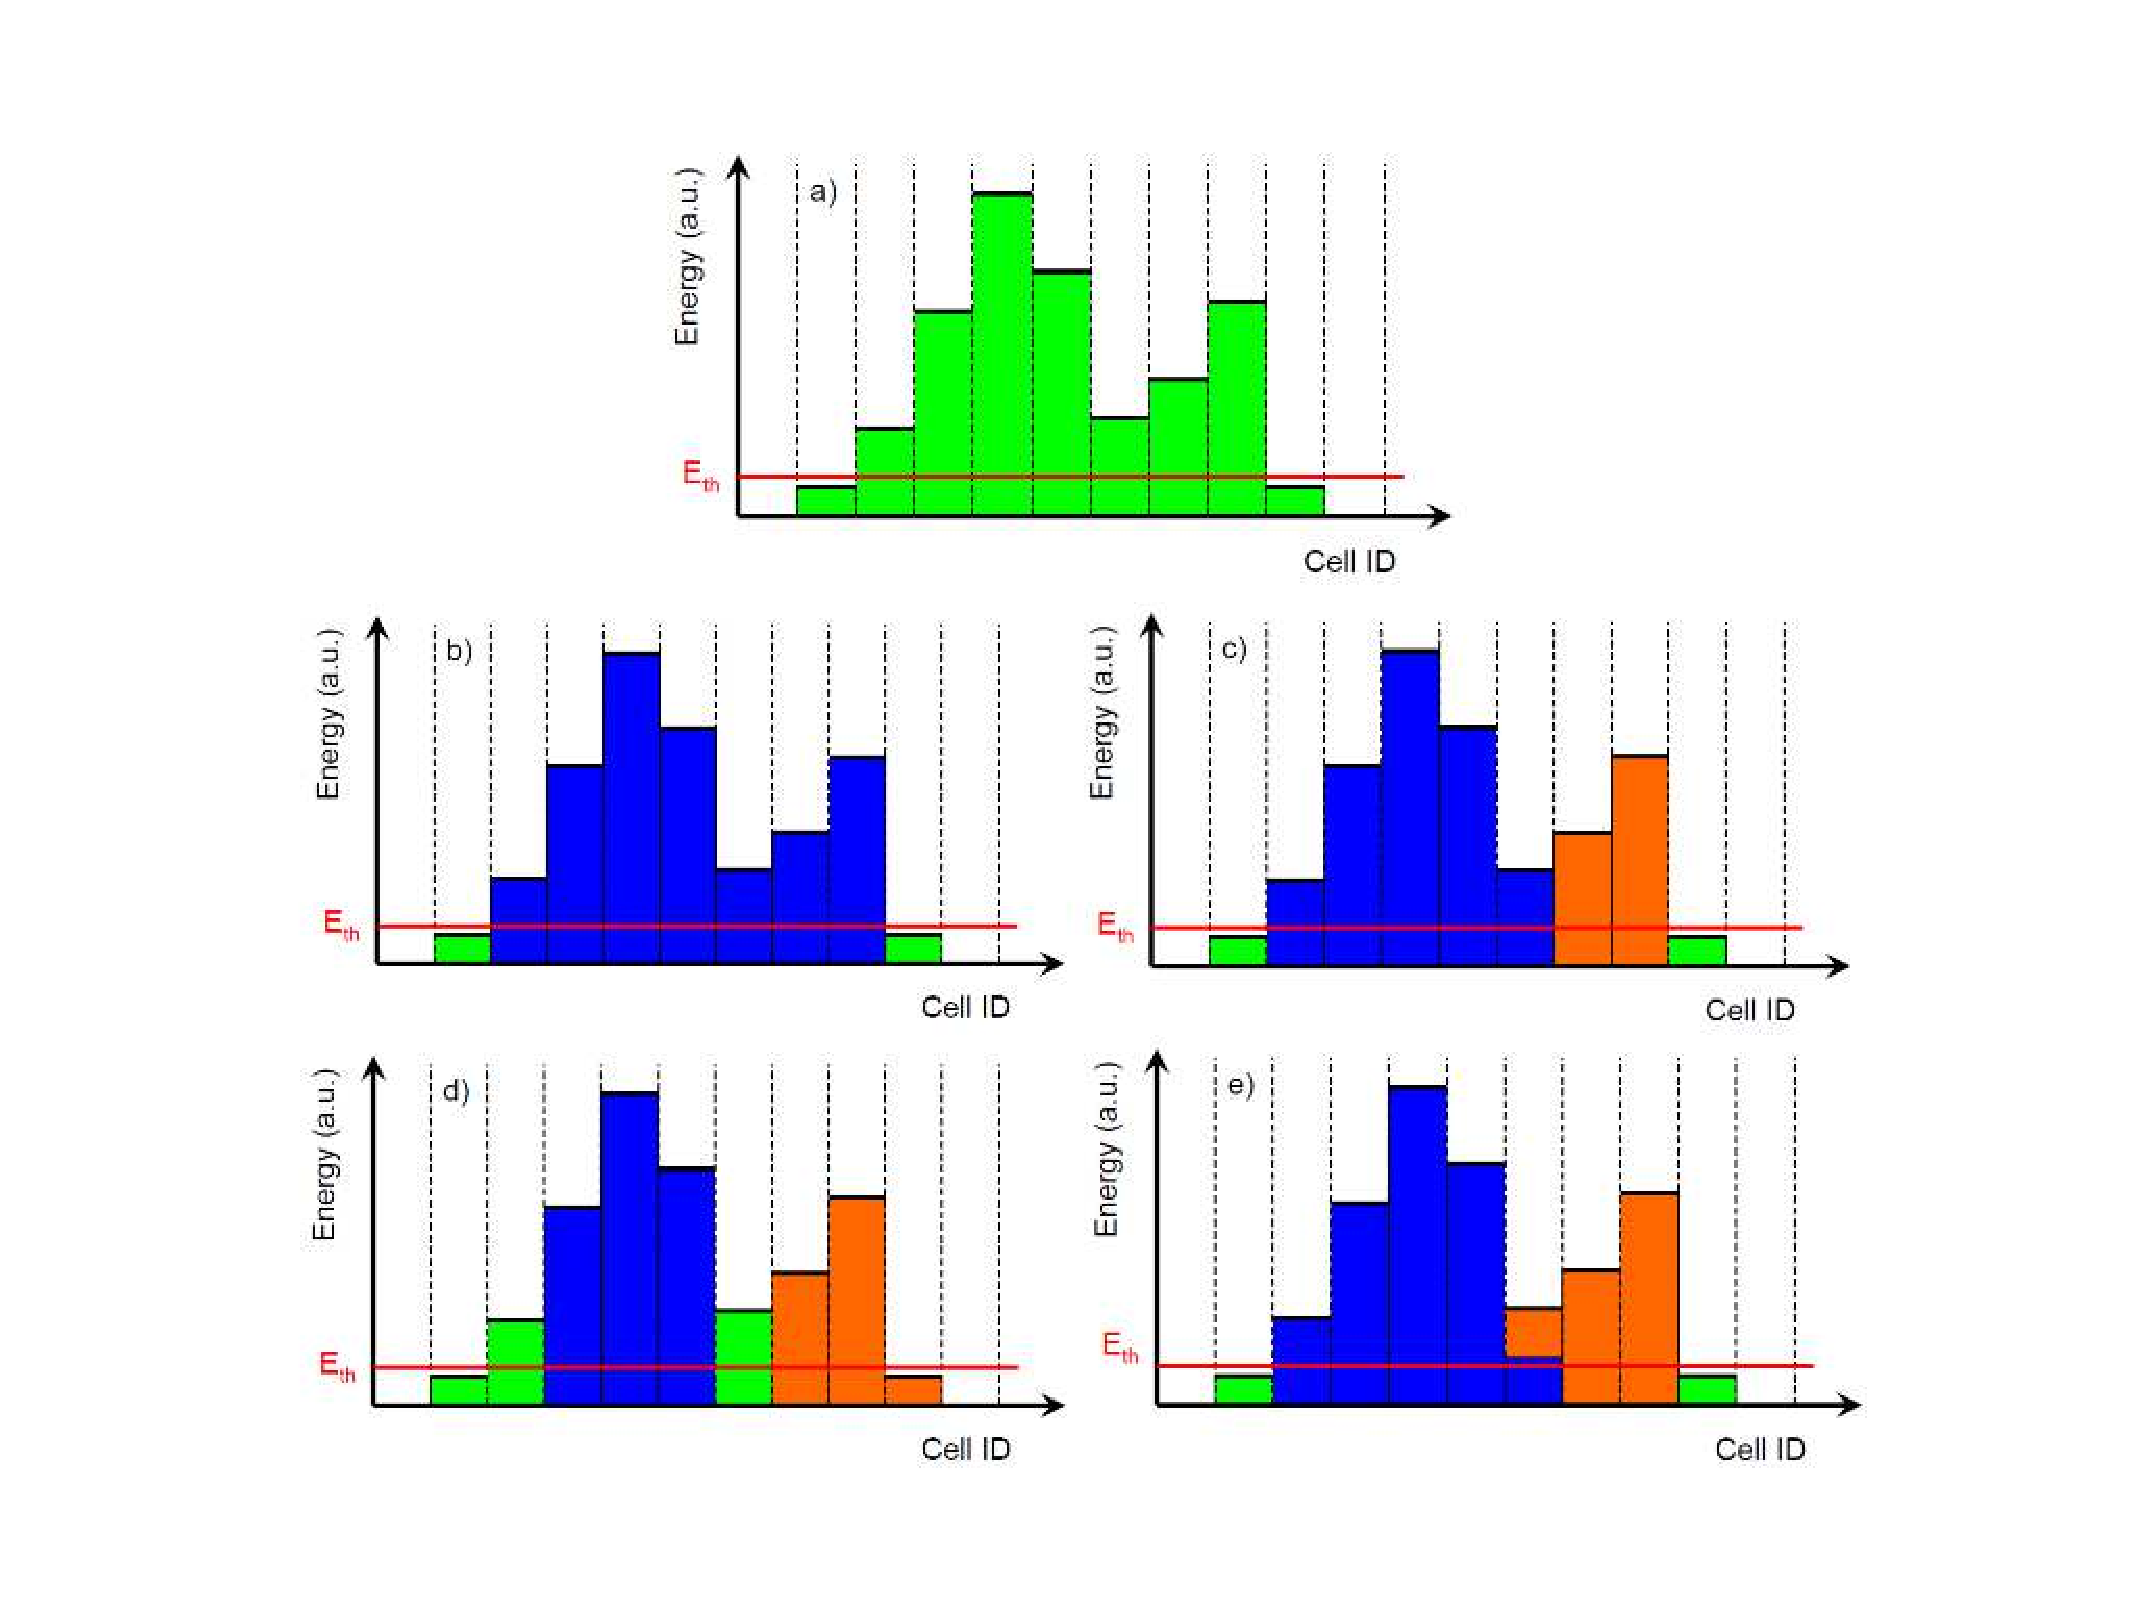
\includegraphics[scale=0.4]{figures/clusters}
\caption{Comparison of different algorithms of clusterization. Boxes represent energy in cells. $E_{th}$ is clusterization threshold \texttt{fMinECut}. a) Energy in cells before clusterization marked by green color. b) Result of V1 clusterizer. There is one big cluster made of cells in blue color. Green cells are below threshold and not associated to the cluster. c) Result of V2 algorithm. There are two clusters made of blue and orange cells. Green cells are below threshold and not associated to any cluster. d) Result of NxN clusterizer. There are two clusters made of blue and orange cells. Green cells are not associated to any cluster. e) Result of V1 algorithm with unfolding. There are two clusters made of blue and orange cells. One cell is associated to two clusters and its energy is shared. Green cells are below threshold and not associated to any cluster. }
\label{fig:clusterizers}
\end{center}
\end{figure}

\subsubsection{Clusterizer NxN}
%The initial step in this algorithm is a calibration of each digit to obtain the ``working array'' of digits (pool of digits). It is the same like for V1 clusterizer. 
The highest energy digit which exceeds energy threshold \texttt{fMinECut} is looked for in the pool of digits. This digit is a seed for a new precluster. To form a precluster we loop over remaining digits and check whether they are neighbours of the seed digit. The energy of a neighbour should be smaller than the energy of the seed. Here neighbours are defined in the other way than in the V1 clusterizer: row index difference or column index difference must be less or equal 1. In such requirement one cell can have eight neighbours at maximum. Here neighbours must fulfill also timing condition. The absolute value of time difference for two digits must be less or equal \texttt{fTimeCut}. The precluster starts to be a cluster only if a precluster energy is larger than clustering threshold given by \texttt{fECAClusteringThreshold}. If the requirement is satisfied a new cluster is formed from the precluster and digits which belong to precluster are removed from the pool of digits. Otherwise only the seed digit is removed from the pool of digits. The procedure is repeated but with a new seed if available. Here maximum size of a cluster is $3 \times 3$ cells. However, digits associated to the cluster do not fulfill the energy threshold condition (energy of digit greater than \texttt{fMinECut}). The special case when cluster is formed from digits in two super-modules at the same SM-$\phi$ angle is also supported.

Different methods of clusterization are compared in Fig.~\ref{fig:clusterizers}.

\subsubsection{Cluster in the EMCal}
A cluster is represented by the \texttt{AliEMCALRecPoint} class. This class contains an information about cluster itself (energy, multiplicity, local or global position, etc.), features of the cluster (shower ellipse axes, dispersion, etc.) and digits belonging to the cluster (index, energy, etc.). The list of important fields is shown in Tab.~\ref{tab:recpoint}.
%
\begin{table}[!h]
\begin{center}
  \begin{tabular}{| c | c | l |}
  \hline
  Name & Type & Explanation \\ 
  \hline
	fAmp              &  \texttt{Float\_t  }  &  summed amplitude of digits   \\
	fIndexInList      &  \texttt{Int\_t    }  &  the index of this RecPoint in the\\
                          &                       &  list stored in TreeR (to be set by analysis)\\
	fGlobPos          &  \texttt{TVector3 }   &  global position\\
	fLocPos           &  \texttt{TVector3 }   &  local  position in the sub-detector coordinate\\
	fMulDigit         &  \texttt{Int\_t    }  &  total multiplicity of digits       \\
	fMulTrack         &  \texttt{Int\_t    }  &  total multiplicity of tracks\\
	fDigitsList       &  \texttt{Int\_t*}     & [fMulDigit] list of digit's indexes from which the point was reconstructed\\
	fTracksList       &  \texttt{Int\_t*}     & [fMulTrack] list of tracks to which the point was assigned\\
	fClusterType      &  \texttt{Int\_t    }  &  type of cluster stored: v1\\
        fCoreEnergy       &  \texttt{Float\_t  }  &  energy in a shower core \\
	fLambda[2]        &  \texttt{Float\_t  }  &  shower ellipse axes\\
	fDispersion       &  \texttt{Float\_t  }  &  shower dispersion\\
	fEnergyList       &  \texttt{Float\_t*}   & [fMulDigit] energy of digits\\
	fAbsIdList        &  \texttt{Int\_t*}     & [fMulDigit] absId  of digits\\
	fTime             &  \texttt{Float\_t  }  &  Time of the digit with maximal energy deposition\\
	fNExMax           &  \texttt{Short\_t  }  &  number of (Ex-)maxima before unfolding\\
	fCoreRadius       &  \texttt{Float\_t  }  &  The radius in which the core energy is evaluated\\
	fDETracksList     &  \texttt{Float\_t*}   & [fMulTrack] list of tracks to which the point was assigned\\
	fMulParent        &  \texttt{Int\_t    }  &  Multiplicity of the parents\\
	fMaxParent        &  \texttt{Int\_t    }  &  Maximum number of parents allowed\\
	fParentsList      &  \texttt{Int\_t*}     &  [fMulParent] list of the parents of the digits\\
	fDEParentsList    &  \texttt{Float\_t*}   &  [fMulParent] list of the parents of the digits\\
	fSuperModuleNumber&  \texttt{Int\_t    }  &  number identifying super-module containing recpoint, reference is cell \\
& & with maximum energy\\
	fDigitIndMax      &  \texttt{Int\_t    }  &  Index of digit with max energy in array fAbsIdList\\
	fDistToBadTower   &  \texttt{Float\_t  }  &  Distance to nearest bad tower\\
	fSharedCluster    &  \texttt{Bool\_t   }  &  States if cluster is shared by 2 super-modules in same phi rack (eg. 0,1)\\
	\hline
  \end{tabular}
\end{center}
\caption{Basic fields in the \texttt{AliEMCALRecPoint} class.}
\label{tab:recpoint}
\end{table}
%
\clearpage




\subsection{Cluster-Track matching - Rongrong, Shingo, Michael}

Even though EMCal is intended to measure the energy of particles that interact with EMCal via electromagnetic showering, e.g. photons and electrons, charged hadrons can also deposit energy in EMCal, most commonly via minimum ionization, but also via nuclear interactions generating hadronic showers. In the analysis where the distinction between hadroic and electromagnetic showers is necessary, cluster-track matching is often used to meet this requirement. 

The main method used to extrapolate tracks in the ALICE software framework is:

\begin{DDbox}{\linewidth}
\begin{lstlisting}
 static Bool_t PropagateTrackToBxByBz(AliExternalTrackParam *track, Double_t x, Double_t m,Double_t maxStep, Bool_t rotateTo=kTRUE, Double_t maxSnp=0.8,Int_t sign=0, Bool_t addTimeStep=kFALSE); 
\end{lstlisting}
\end{DDbox}
which takes the following arguments: {\it ``track''} stores all the information of the starting point for the extrapolation; {\it ``x''} is the coordinate of the destination plane in the local coordinate system; {\it ``m''} is the mass assumption for the track; {\it ``maxStep''} is the step size used in the extrapolation. This method extrapolates the track trajectory to a destination plane in a magnetic field, taking into account the energy loss of the tracks when going through detector materials. However, the energy loss model is tuned for charged hadrons, so it does not work very well for electrons or positions whose primary energy loss process is bremsstrahlung.

For EMCal, the track-cluster matching is done by default in the reconstruction chain and the code is implemented in:

\begin{DDbox}{\linewidth}
\begin{lstlisting}
 AliEMCALTracker::PropagateBack(AliESDEvent* esd)
\end{lstlisting}
\end{DDbox}

The logic of the matching procedure is the following:
\begin{itemize}
\item Check wheter TPC is available in DAQ/reco. See AliEMCALTracker::LoadClusters(). In case there is no TPC, ITS specific extrapolation will be used.
\item Find all the EMCal clusters in the event. See AliEMCALTracker::LoadClusters().
\item Find all the good tracks in the event. See AliEMCALTracker:: LoadTracks(). Several cuts are applied to select good tracks
	\begin{itemize}
	\item Minimum $p_{\rm{T}}$ cut, which can be set during the reconstruction.
	\item Cut on number of TPC clusters, which can be set during the reconstruction. This specific cut is avoided in case there is only ITS available in reconstruction. 	
	\item $|\eta|<0.8$ and $20^{\circ} < \varphi < 120^{\circ} $. These fiducial cuts are hard coded since tracks out of this range should never make it to EMCal. 
	\end{itemize}
\item For each good track, find the nearest cluster as matched if their residuals fall within the cuts. See AliEMCALTracker::FindMatchedCluster(), which follows the following steps:
	\begin{itemize}
	\item Get the starting point: if the {\it friendTrack} is available, use the last point on the TPC. Otherwise, use the point at the inner wall of the TPC.
	\item If only ITS tracks are available in reconstruction, the propagation will use the track information from the vertex.  	   
	\item Extrapolate tracks to the EMCal surface at 430 cm, and apply fiducial cuts on the extrapolated points: $|\eta|<0.75$ and $70^{\circ} < \varphi < 190^{\circ} $. The step size in the extrapolation can be set in the reconstruction, and the default value is 20 cm.
	\item Extrapolate tracks further, with 5 cm step size, to the positions of all the EMCal clusters which are in the vicinity of the extrapolated points from last step. Then the distance between extrapolated tracks to the clusters are calculated, and the nearest cluster is assigned as matched if the residuals fall within cuts. By fitting the distributions of the residuals using Gaussian functions, we can choose to cut on $N\sigma$ of the residuals.To further improve the matching performance, $p_{\rm{T}}$ and charge dependent cuts can be used. 
	\end{itemize}
\end{itemize}



\subsection{How to execute the reconstruction}

Executing the reconstruction is very similar to the simulation case, see the macro TestEMCALReconstruction.C (a bit more detailed than the one in \$ALICE\_ROOT/EMCAL/macros) :

\begin{DDbox}{\linewidth}
\begin{lstlisting}
void TestEMCALReconstruction() {

TString detector=``EMCAL TPC'';//Same function as in Simulation.C  
// TString detector=``EMCAL ITS''; if user wants ITS tracking to be used.

AliReconstruction rec; //Create reconstruction object 

//Making Tracking 
rec.SetRunTracking(detector) ;

//Particle Reconstruction. Make Rec Points 
rec.SetRunReconstruction(detector); 

//read RAW data. Give directory where raw data is stored
//rec.SetInput(``RawDataDirectory/raw.root");

//Make vertex finder 
rec.SetRunVertexFinder(kFALSE) ; // false only if the tracking detectors are not included.

//Fill ESD file with RecPoints information. 
rec.SetFillESD(detector) ; 

//Run Reconstruction 
rec.Run() ;
}
\end{lstlisting}
\end{DDbox}


